%! Author = adrien koumgang tegantchouang
%! Date = 09/07/24


\chapter{Benchmarking}\label{ch:benchmarking}

The performance tests will be carried out on three implementations: SageMath's, Pistiloglou's and my own.
To do this, I have chosen an approach that consists of calculating the time needed to perform the modular decomposition of a graph over two groups of graphs.
The first group is made up of so-called small graphs, where the number of nodes is of the order of ten.
These are mainly the graphs discussed in the theory in Chapter~\ref{ch:modular-decomposition}.
The second group is made up of large, undirected, randomly generated graphs.
For this group, the number of nodes is on the order of multiples of hundreds.

\section{Development and test environment}\label{sec:development-and-test-environment}

To write the code and run the tests, I'm using a MacBook Pro of Apple with an M2 processor, 8GB of RAM and 512GB of ROM\cite{macbookprom2}.

\subsection{Development environment: RustRover}\label{subsec:development-environment-rustrover}

RustRover\cite{rustrover} by JetBrains\cite{jetbrains} is the chosen IDE for this project due to its powerful features tailored for Rust development.
It provides advanced code navigation, refactoring tools, debugging capabilities, and seamless integration with Rust's toolchain.
This environment allows for efficient handling of both small and large Rust projects, making it ideal for modular decomposition.

Key features of RustRover that support this project:
\begin{itemize}
    \item \textbf{Intelligent Code Assistance:} Code completion, suggestions, and real-time analysis.
    \item \textbf{Cargo Integration:} RustRover's deep integration with Cargo enables seamless management of dependencies, builds, and test runs.
    \item \textbf{Debugging:} Powerful debugger that supports breakpoints, variable inspection, and expression evaluation.
    \item \textbf{Version Control Integration:} Built-in Git and GitHub integration to handle version control without leaving the IDE\@.
    \item \textbf{Test Runner:} Simplifies the process of writing and running unit tests using Rust’s built-in test framework.
\end{itemize}

\subsection{Test environment and benchmarking}\label{subsec:test-environment-and-benchmarking}

The graphs on which the tests were carried out were generated at random using the following Python code and saved in .dot files which are then read by each implementation.

\begin{lstlisting}[language=Python, style=python, caption={Graph generation code}, label={lst:graph-generation-code}, firstnumber=1]
    import random

    from twostructure import TwoStructure


    def generate_graph_twostructure(n, p=0.1):
        import random
        ts = TwoStructure()
        for i in range(n):
            for j in range(i + 1, n):
                if random.random() < p:  # Add edges with probability p
                    ts.uedge(i, j)

        return ts
\end{lstlisting}


\subsubsection{Python tool for test benchmarking: pytest-benchmark}

Pytest-benchmark\cite{pytestbenchmark} is a plugin for the pytest framework that allows developers to benchmark the performance of their code.
It helps measure execution time and detect performance regressions across test runs.
Key features of pytest-benchmark include:
\begin{enumerate}
    \item \textbf{Performance Testing:} Easily measure and compare the speed of code sections or functions, providing detailed performance metrics like min, max, mean, and standard deviation of execution time.
    \item \textbf{Comparison:} Track and compare benchmark results over time to detect any performance regressions or improvements.
    \item \textbf{Customizable:} Users can control warm-up times, repetitions, and iterations to fine-tune the precision and accuracy of the benchmarks.
    \item \textbf{Reporting:} pytest-benchmark generates detailed, human-readable reports with performance data, which can be saved to files (JSON, CSV) for further analysis or CI integration.
    \item \textbf{Command-Line Integration:} Benchmarking results can be viewed and compared directly from the command line.
    \item \textbf{Integration with pytest:} pytest-benchmark fits seamlessly into existing pytest test suites, so you can combine functional testing with performance benchmarks.
\end{enumerate}


\subsubsection{Rust tool for test benchmarking: Criterion}

Criterion\cite{criterion} is a powerful and flexible benchmarking framework for Rust, which provides statistically rigorous and reliable performance metrics.
Criterion.rs benchmarks collect and store statistical information from run to run and can automatically detect performance regressions as well as measuring optimizations.
It helps to measure the performance of various code sections, especially critical algorithms like those used in this project for modular decomposition of graphs.

Criterion was chosen for this project due to its advanced features, including:
\begin{itemize}
    \item \textbf{Statistical Significance:} It ensures that the benchmarking results are reliable by conducting statistical analysis of the timings.
    \item \textbf{Visual Reports:} Criterion generates detailed reports in both text and HTML formats, allowing for easy interpretation of results.
    \item \textbf{Comparative Benchmarking:} It allows comparing current benchmarks with previous runs to track performance improvements or regressions.
    \item \textbf{Ease of Use:} Criterion integrates well with Cargo, making it simple to run benchmarks alongside tests.
\end{itemize}

The benchmarks focus on measuring the performance of key functions in the modular decomposition algorithm.
The Criterion framework is used to evaluate execution time, memory usage, and other metrics across different input sizes and graph configurations.

To set up Criterion for this project, the following steps were followed:
\begin{enumerate}
    \item Add Criterion as a development dependency in `Cargo.toml'
    \item  Create a `benches' directory in the project root, and add a new Rust file, typically named `benchmark.rs'.
    This file contains the benchmarking code.
    \item Ensure that benchmarks are placed in the `benches' directory, as Criterion uses the convention of placing benchmarks outside the main `src' directory to avoid them being compiled into the release builds.
\end{enumerate}

\begin{myex}[Example Benchmark Code for Rust]

\end{myex}

\begin{lstlisting}[language=Rust, style=rust, caption={Example of benchmark code for modular decomposition}, label={lst:rust-example-of-benchmark-code}, firstnumber=1]
    use std::hint::black_box;
    use criterion::{criterion_group, criterion_main, Criterion};

    use moddecomp::two_structure::{graph_ex1, TwoStructure};
    use moddecomp::moddecomp::moddecomp::modular_decomposition;


    fn criterion_benchmark(c: &mut Criterion) {
        c.bench_function("modular decomposition graph ex1", |b| b.iter(|| modular_decomposition(black_box(&mut graph_ex1()), black_box(None))));
    }

    criterion_group!(benches, criterion_benchmark);
    criterion_main!(benches);
\end{lstlisting}

\begin{itemize}
    \item \textbf{black\_box:} Ensures that the Rust compiler does not optimize away the benchmarked code, providing more accurate results.
    \item \textbf{criterion\_group and criterion\_main:} These macros register the benchmarks and allow Criterion to execute them.
\end{itemize}

Once Criterion is configured, benchmarks can be run using Cargo: `cargo bench'.
This command will execute the benchmarks, and Criterion will output the results in the terminal.
It will also generate more detailed reports in the `target/criterion' directory, including both text summaries and HTML reports for visual analysis.

The benchmarks are designed to evaluate the following:
\begin{itemize}
    \item \textbf{Execution Time:} How long it takes for the modular decomposition algorithm to run on different types and sizes of graphs.
    \item \textbf{Scalability:} How the algorithm’s performance changes as the size and complexity of the graph input increase.
    \item \textbf{Comparative Performance:} How different versions of the algorithm or alternative approaches perform relative to each other.
\end{itemize}

Benchmarks are run with multiple iterations and warm-up phases to ensure accuracy.
Criterion’s statistical analysis methods (including bootstrapping) are used to minimize variance and provide a robust estimate of the true performance characteristics.

\begin{myex}[Example output]
    For the tests, we will be looking mainly at two output results:
    \begin{enumerate}
        \item \textbf{Terminal Output:}
                \begin{figure}[!h]
                    \centering
                    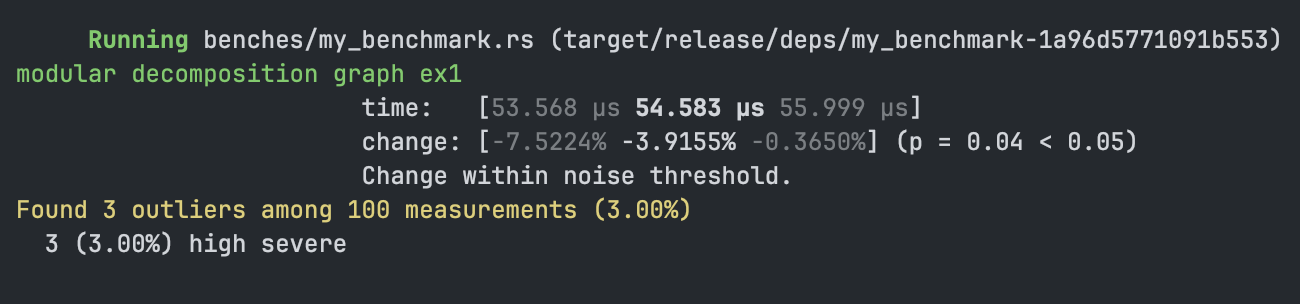
\includegraphics[width=0.80\textwidth]{images/benchmark/benchmark-terminal-output}
                    \caption{Example of Terminal ouput for modular decomposition of graph ex1}
                    \label{fig:example-of-terminal-output}
                \end{figure}
        \item \textbf{HTML Reports:}
                \begin{figure}[!h]
                    \centering
                    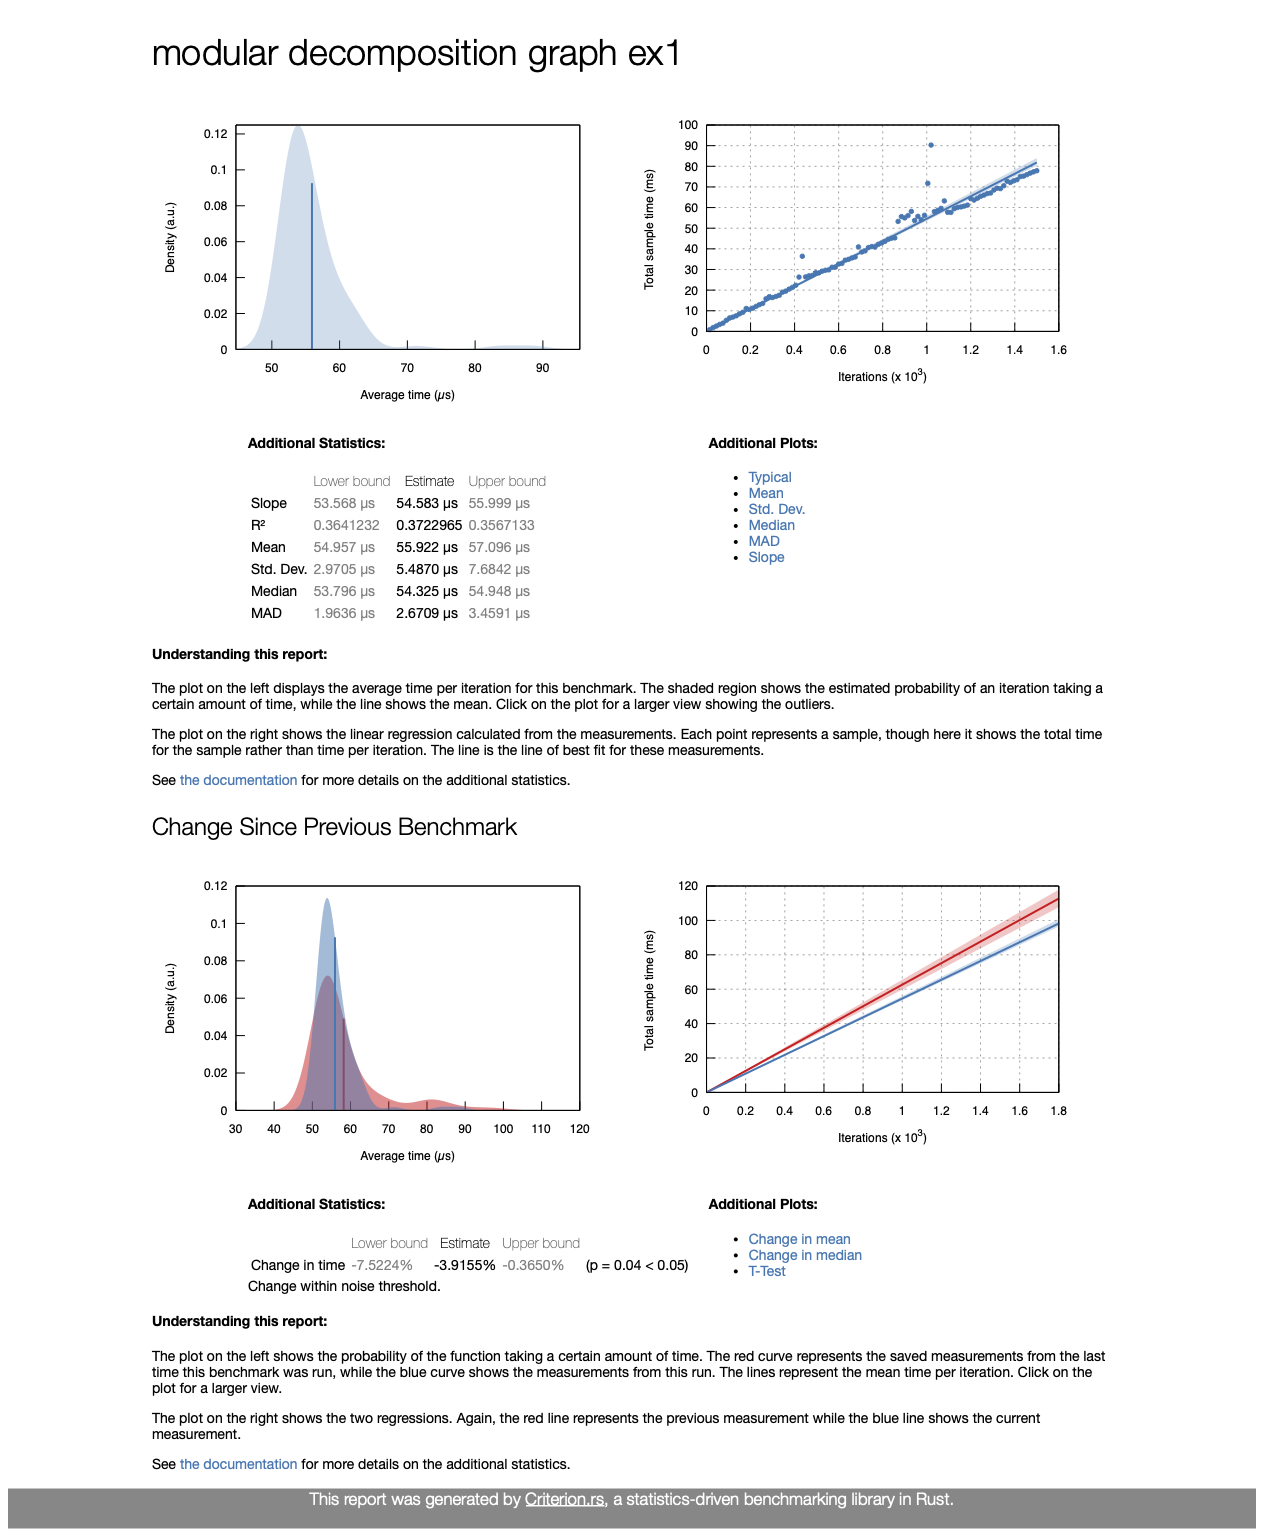
\includegraphics[width=1\textwidth]{images/benchmark/benchmark-html-output}
                    \caption{Example of HTML ouput for modular decomposition of graph ex1}
                    \label{fig:example-of-html-output}
                \end{figure}
    \end{enumerate}
\end{myex}


\subsubsection{Python code for test benchmarking SageMath implementation}

Unfortunately, I haven't found a tool that lets me run benchmark tests directly in SageMath.
To replicate the style of results we get from Criterion in Rust and pytest-benchmark in Pythib, I use the following approach in SageMath:
\begin{itemize}
    \item \textbf{Multiple Timings and Averages:} Run the code multiple times to get an average execution time.
    \item \textbf{Statistical Reporting:} Report min, max, and mean execution times, along with standard deviation, similar to Criterion’s output.
\end{itemize}

\begin{myex}[Example Benchmark Code SageMath]

\end{myex}

\begin{lstlisting}[language=Python, style=python, caption={Example of benchmark code for modular decomposition}, label={lst:sagemath-example-of-benchmark-code}, firstnumber=1]
    import time
    import numpy as np

    def benchmark_modular_decomposition(graph, iterations=100):
        times = []

        for _ in range(iterations):
            # Start timer
            start_time = time.time()

            # Perform the computation
            graph.modular_decomposition()

            # Stop timer
            end_time = time.time()

            # Record execution time in microseconds (µs)
            execution_time = (end_time - start_time)
            times.append(execution_time)

        # Calculate benchmark statistics using NumPy
        min_time = np.min(times)
        max_time = np.max(times)
        mean_time = np.mean(times)
        stdev_time = np.std(times)

        # Print results in seconds (s)
        print(f"Benchmark Results (over {iterations} iterations) in s:")
        print(f"Min Time: {min_time:.2f} s")
        print(f"Max Time: {max_time:.2f} s")
        print(f"Mean Time: {mean_time:.2f} s")
        print(f"Standard Deviation: {stdev_time:.2f} s")
\end{lstlisting}


\section{Result for small graphs}\label{sec:result-for-small-graphs}

Let's start with the first test on the graph in Figure\ref{fig:example-undirected-graph} and in Figure\ref{fig:example-directed-graph}.
Here it's called a small graph because of its size, containing just 11 nodes for the first graph and 8 for the second.

\newpage

\subsection{Benchmark for simple undirected graph\ref{fig:example-undirected-graph}}\label{subsec:benchmark-for-simple-undirected-graph}

\subsubsection*{SageMath implementation}
\begin{figure}[!h]
    \centering
    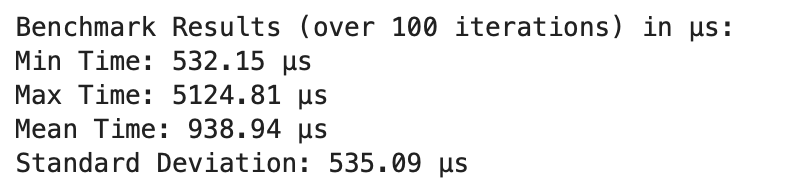
\includegraphics[width=0.40\textwidth]{images/benchmark/graph_wikipedia/benchmark_graph_wikipedia_sagemath}
    \caption{Result benchmark SageMath implementation}
    \label{fig:benchmark-graph-wikipedia-sagemath}
\end{figure}

\subsubsection*{Eleni Pistiloglou's implementation}
\begin{figure}[!h]
    \centering
    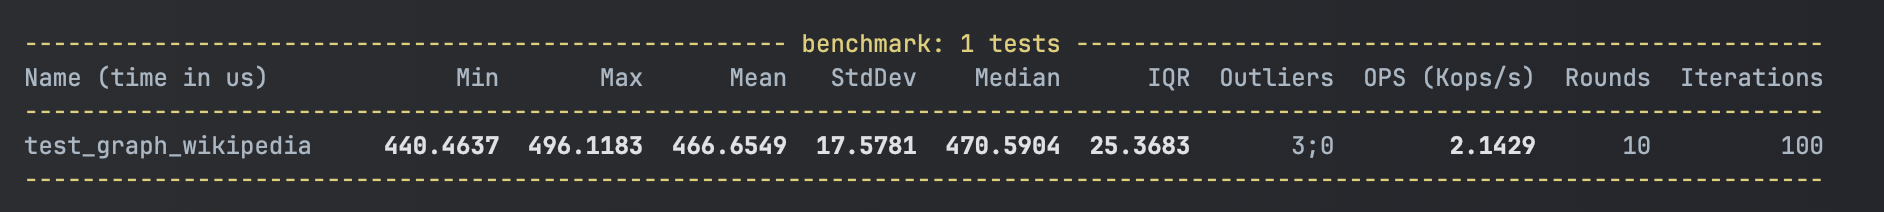
\includegraphics[width=0.60\textwidth]{images/benchmark/graph_wikipedia/benchmark_graph_wikipedia_python}
    \caption{Result benchmark Eleni Pistiloglou's implementation}
    \label{fig:benchmark-graph-wikipedia-python}
\end{figure}

\subsubsection*{Rust implementation}
\begin{figure}[!h]
    \centering
    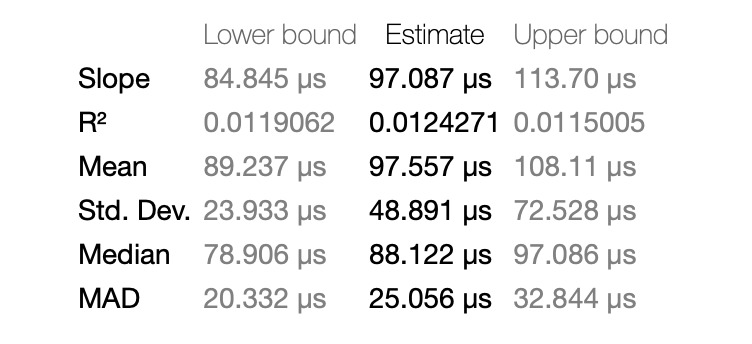
\includegraphics[width=0.40\textwidth]{images/benchmark/graph_wikipedia/benchmark_graph_wikipedia_rust}
    \caption{Result benchmark Rust implementation}
    \label{fig:benchmark-graph-wikipedia-rust}
\end{figure}

\subsubsection*{Benchmark Comparison}
\begin{figure}[!h]
    \centering
    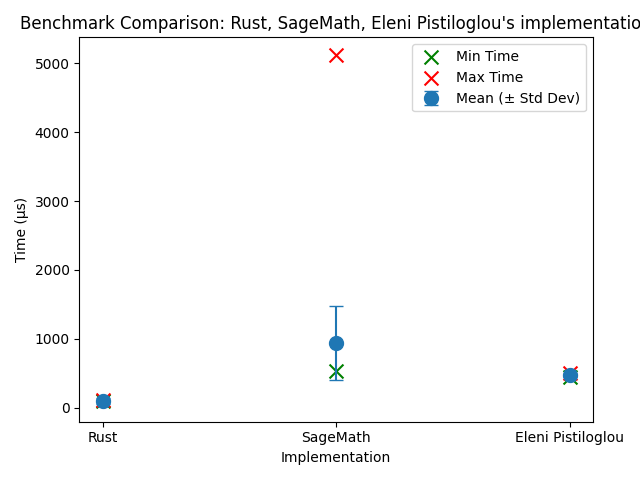
\includegraphics[width=0.40\textwidth]{images/benchmark/graph_wikipedia/benchmark_comparison_graph_wikipedia}
    \caption{Result benchmark Rust implementation}
    \label{fig:benchmark-comparison-graph-wikipedia}
\end{figure}

\newpage

\subsection{Benchmark for simple directed graph\ref{fig:example-directed-graph}}\label{subsec:benchmark-for-simple-directed-graph}

\subsubsection*{SageMath implementation}
\begin{figure}[!h]
    \centering
    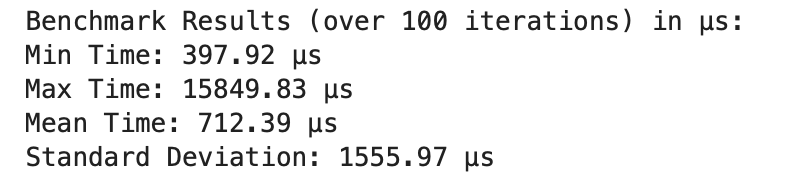
\includegraphics[width=0.40\textwidth]{images/benchmark/digraph/benchmark_digraph_sagemath}
    \caption{Result benchmark SageMath implementation}
    \label{fig:benchmark-digraph-sagemath}
\end{figure}

\subsubsection*{Eleni Pistiloglou's implementation}
\begin{figure}[!h]
    \centering
    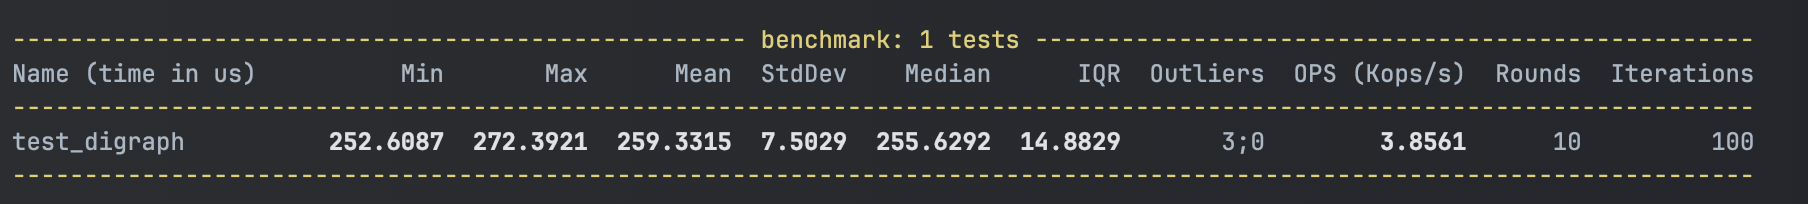
\includegraphics[width=0.60\textwidth]{images/benchmark/digraph/benchmark_digraph_python}
    \caption{Result benchmark Python implementation}
    \label{fig:benchmark-digraph-python}
\end{figure}

\subsubsection*{Rust implementation}
\begin{figure}[!h]
    \centering
    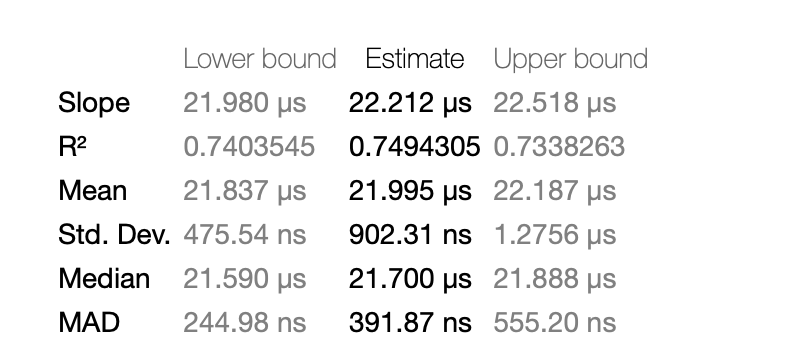
\includegraphics[width=0.40\textwidth]{images/benchmark/digraph/benchmark_digraph_rust}
    \caption{Result benchmark Rust implementation}
    \label{fig:benchmark-digraph-rust}
\end{figure}

\subsubsection*{Benchmark Comparison}
\begin{figure}[!h]
    \centering
    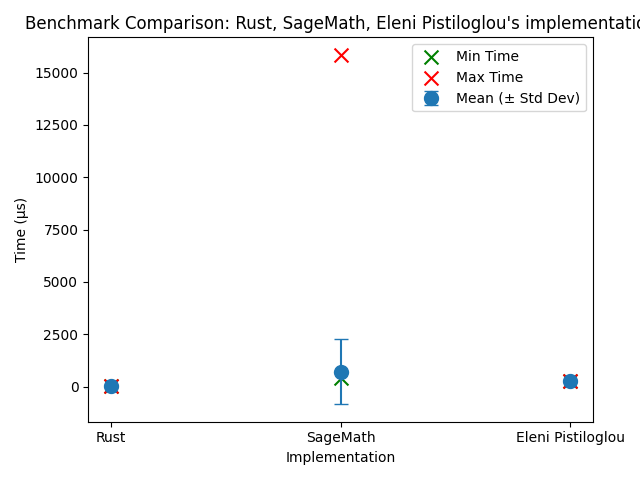
\includegraphics[width=0.40\textwidth]{images/benchmark/digraph/benchmark_comparison_digraph}
    \caption{Result benchmark Rust implementation}
    \label{fig:benchmark-comparison-digraph}
\end{figure}


\newpage


\section{Result for large graphs}\label{sec:result-for-large-graphs}

\subsection{100 nodes and 1058 edges}\label{subsec:result-for-graphs-100-1058}

\subsubsection*{SageMath implementation}
\begin{figure}[!h]
    \centering
    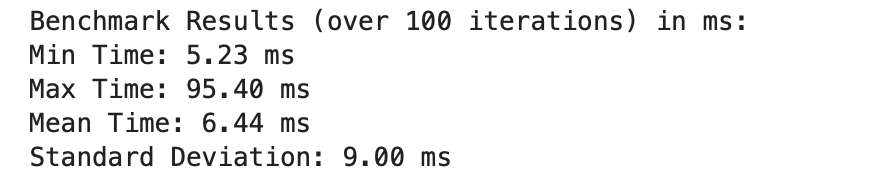
\includegraphics[width=0.40\textwidth]{images/benchmark/large_graph/benchmark_large_graph_sagemath}
    \caption{Result benchmark SageMath implementation}
    \label{fig:benchmark-large-graph-sagemath}
\end{figure}

\subsubsection*{Eleni Pistiloglou's implementation}
\begin{figure}[!h]
    \centering
    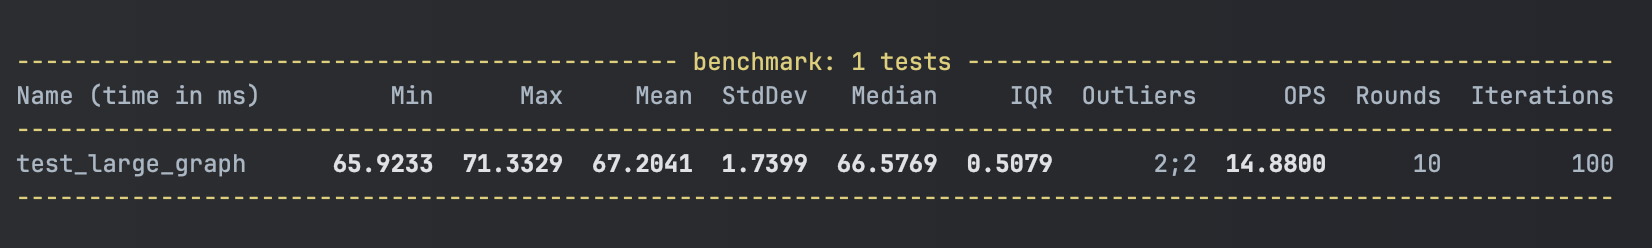
\includegraphics[width=0.50\textwidth]{images/benchmark/large_graph/benchmark_large_graph_python}
    \caption{Result benchmark Eleni Pistiloglou's implementation}
    \label{fig:benchmark-large-graph-python}
\end{figure}

\subsubsection*{Rust implementation}
\begin{figure}[!h]
    \centering
    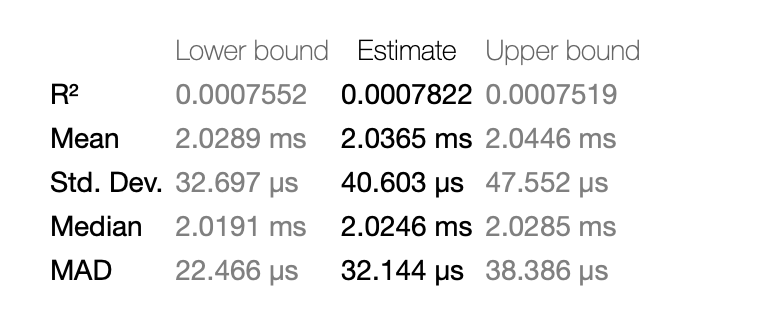
\includegraphics[width=0.40\textwidth]{images/benchmark/large_graph/benchmark_large_graph_rust}
    \caption{Result benchmark Rust implementation}
    \label{fig:benchmark-large-graph-rust}
\end{figure}

\subsubsection*{Benchmark Comparison}
\begin{figure}[!h]
    \centering
    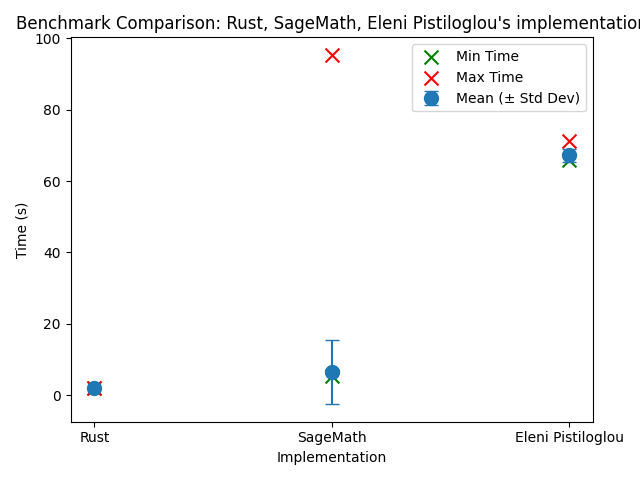
\includegraphics[width=0.35\textwidth]{images/benchmark/large_graph/benchmark_comparison_graph_100_1058}
    \caption{Result benchmark Rust implementation}
    \label{fig:benchmark-comparison-graph-100-1058}
\end{figure}


\newpage


\subsection{100 nodes and 970 edges}\label{subsec:result-for-graphs-100-970}

\subsubsection*{SageMath implementation}
\begin{figure}[!h]
    \centering
    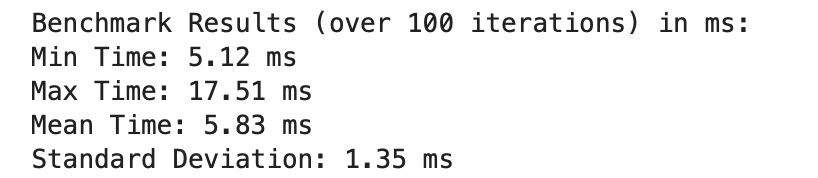
\includegraphics[width=0.40\textwidth]{images/benchmark/graph_100_970/benchmark_graph_100_970_sagemath}
    \caption{Result benchmark SageMath implementation}
    \label{fig:benchmark-graph-100-970-sagemath}
\end{figure}

\subsubsection*{Eleni Pistiloglou's implementation}
\begin{figure}[!h]
    \centering
    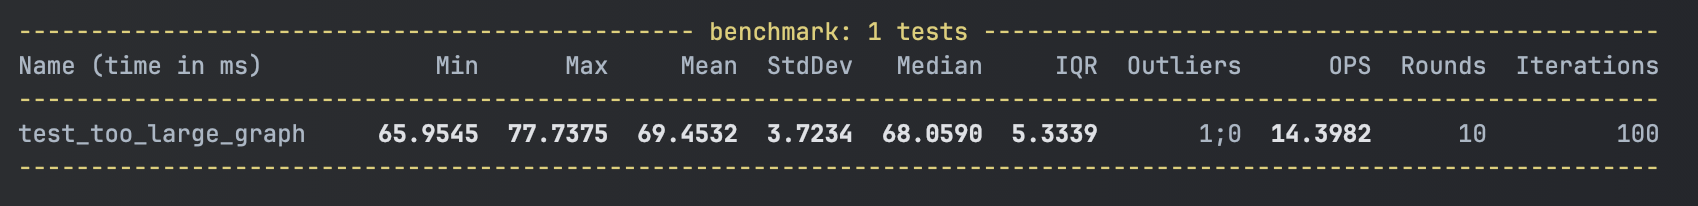
\includegraphics[width=0.60\textwidth]{images/benchmark/graph_100_970/benchmark_graph_100_970_python}
    \caption{Result benchmark Eleni Pistiloglou's implementation}
    \label{fig:benchmark-graph-100-970-python}
\end{figure}

\subsubsection*{Rust implementation}
\begin{figure}[!h]
    \centering
    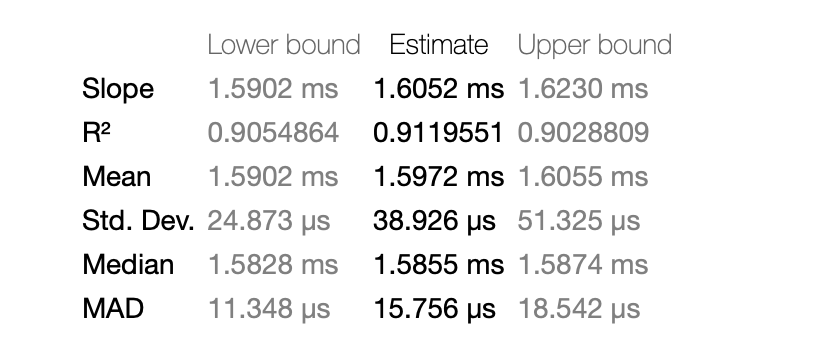
\includegraphics[width=0.40\textwidth]{images/benchmark/graph_100_970/benchmark_graph_100_970_rust}
    \caption{Result benchmark Rust implementation}
    \label{fig:benchmark-graph-100-970-rust}
\end{figure}

\subsubsection*{Benchmark Comparison}
\begin{figure}[!h]
    \centering
    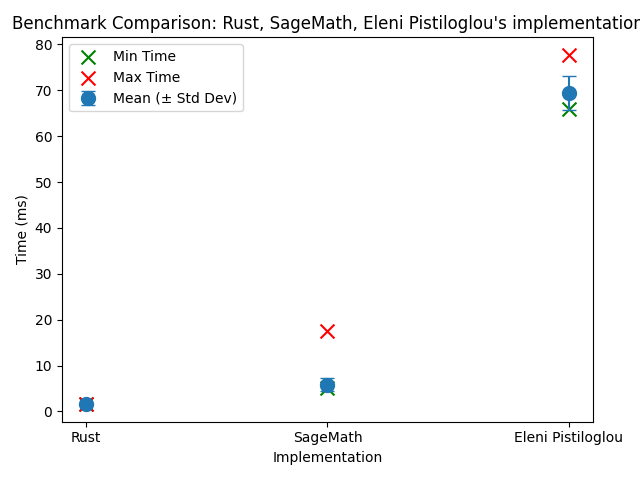
\includegraphics[width=0.40\textwidth]{images/benchmark/graph_100_970/benchmark_comparison_graph_100_970}
    \caption{Result benchmark Rust implementation}
    \label{fig:benchmark-comparison-graph-100-970}
\end{figure}


\newpage


\subsection{200 nodes and 3896 edges}\label{subsec:result-for-graphs-200-3896}

\subsubsection*{SageMath implementation}
\begin{figure}[!h]
    \centering
    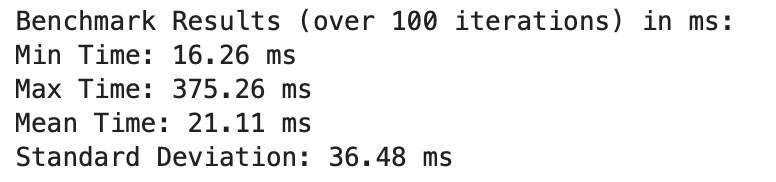
\includegraphics[width=0.40\textwidth]{images/benchmark/graph_200_3896/benchmark_graph_200_3896_sagemath}
    \caption{Result benchmark SageMath implementation}
    \label{fig:benchmark-graph-200-3896-sagemath}
\end{figure}

\subsubsection*{Eleni Pistiloglou's implementation}
\begin{figure}[!h]
    \centering
    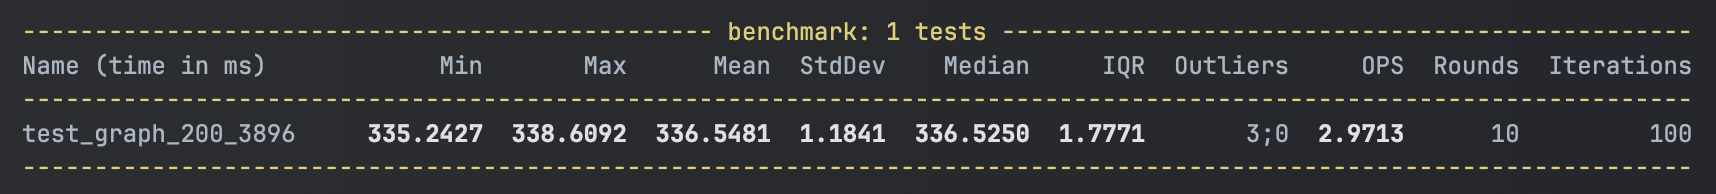
\includegraphics[width=0.60\textwidth]{images/benchmark/graph_200_3896/benchmark_graph_200_3996_python}
    \caption{Result benchmark Eleni Pistiloglou's implementation}
    \label{fig:benchmark-graph-200-3896-python}
\end{figure}

\subsubsection*{Rust implementation}
\begin{figure}[!h]
    \centering
    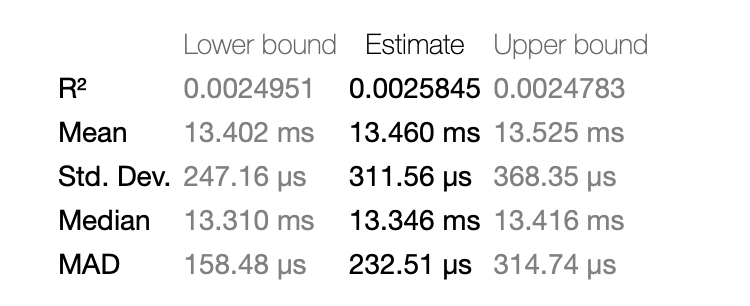
\includegraphics[width=0.40\textwidth]{images/benchmark/graph_200_3896/benchmark_graph_200_3996_rust}
    \caption{Result benchmark Rust implementation}
    \label{fig:benchmark-graph-200-3896-rust}
\end{figure}

\subsubsection*{Benchmark Comparison}
\begin{figure}[!h]
    \centering
    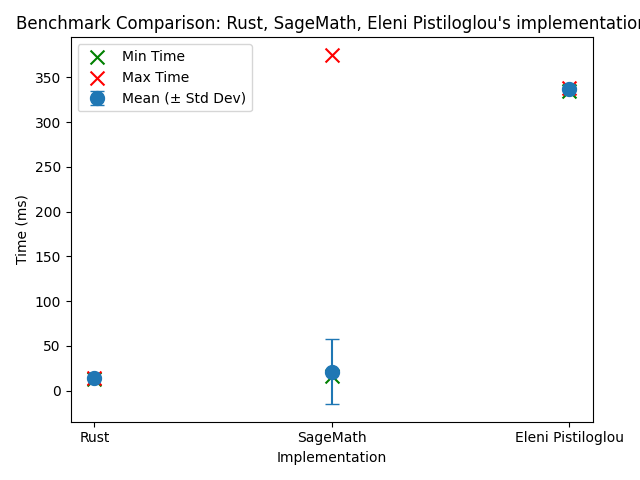
\includegraphics[width=0.40\textwidth]{images/benchmark/graph_200_3896/benchmark_comparison_graph_200_3896}
    \caption{Result benchmark Rust implementation}
    \label{fig:benchmark-comparison-graph-200-3896}
\end{figure}

\newpage


\subsection{200 nodes and 3880 edges}\label{subsec:result-for-graphs-200-3880}

\subsubsection*{SageMath implementation}
\begin{figure}[!h]
    \centering
    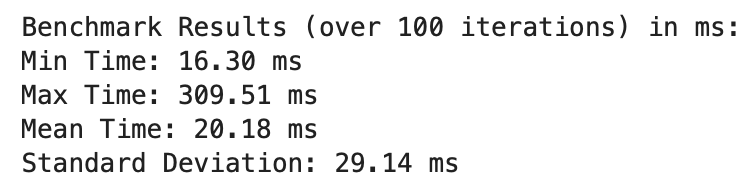
\includegraphics[width=0.40\textwidth]{images/benchmark/graph_200_3880/benchmark_graph_200_3880_sagemath}
    \caption{Result benchmark SageMath implementation}
    \label{fig:benchmark-graph-200-3880-sagemath}
\end{figure}

\subsubsection*{Eleni Pistiloglou's implementation}
\begin{figure}[!h]
    \centering
    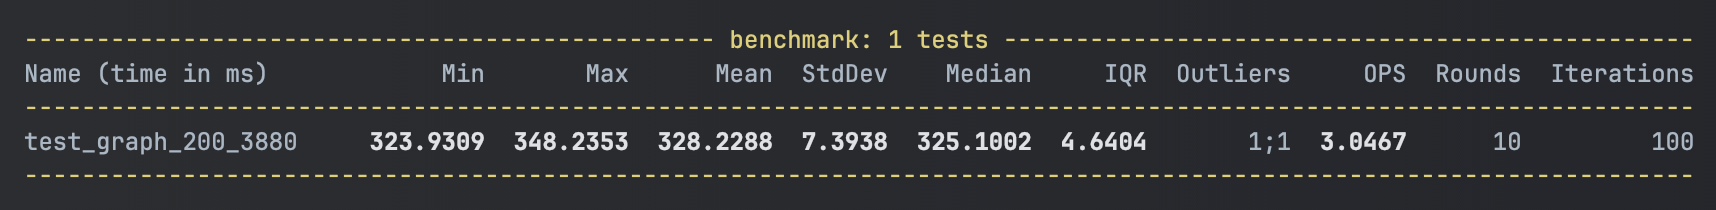
\includegraphics[width=0.60\textwidth]{images/benchmark/graph_200_3880/benchmark_graph_200_3880_python}
    \caption{Result benchmark Eleni Pistiloglou's implementation}
    \label{fig:benchmark-graph-200-3880-python}
\end{figure}

\subsubsection*{Rust implementation}
\begin{figure}[!h]
    \centering
    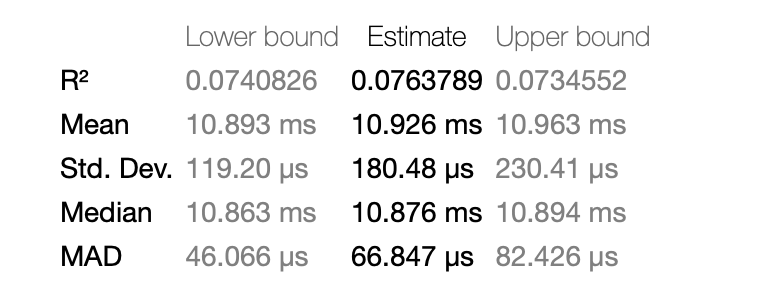
\includegraphics[width=0.40\textwidth]{images/benchmark/graph_200_3880/benchmark_graph_200_3880_rust}
    \caption{Result benchmark Rust implementation}
    \label{fig:benchmark-graph-200-3880-rust}
\end{figure}

\subsubsection*{Benchmark Comparison}
\begin{figure}[!h]
    \centering
    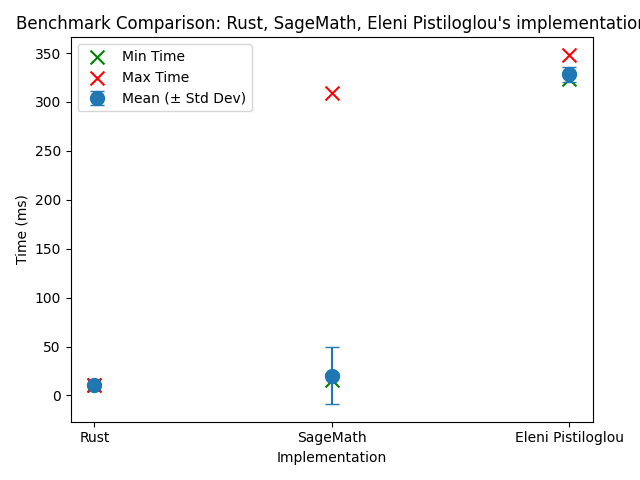
\includegraphics[width=0.40\textwidth]{images/benchmark/graph_200_3880/benchmark_comparison_graph_200_3880}
    \caption{Result benchmark Rust implementation}
    \label{fig:benchmark-comparison-graph-200-3880}
\end{figure}


\newpage

\subsection{500 nodes - 24876 edges}\label{subsec:result-for-graphs-500-24876}

\subsubsection*{SageMath implementation}
\begin{figure}[!h]
    \centering
    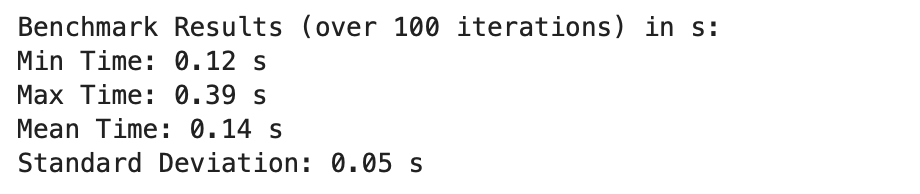
\includegraphics[width=0.40\textwidth]{images/benchmark/too_large_graph/benchmark_too_large_graph_sagemath}
    \caption{Result benchmark SageMath implementation}
    \label{fig:benchmark-graph-500-24876-sagemath}
\end{figure}

\subsubsection*{Eleni Pistiloglou's implementation}
\begin{figure}[!h]
    \centering
    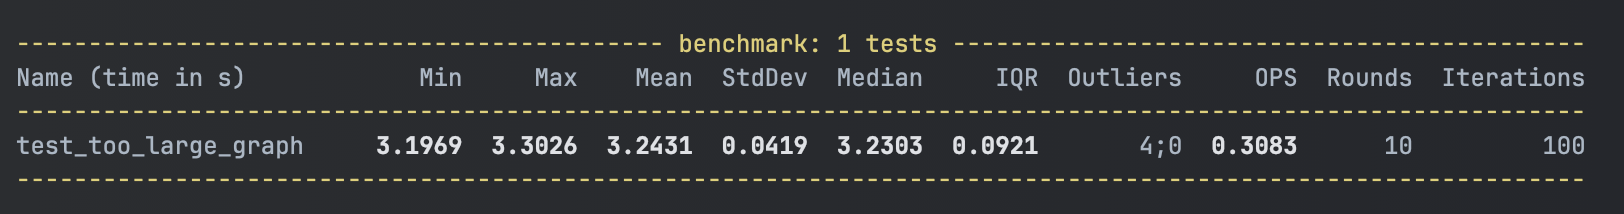
\includegraphics[width=0.60\textwidth]{images/benchmark/too_large_graph/benchmark_too_large_graph_python}
    \caption{Result benchmark Eleni Pistiloglou's implementation}
    \label{fig:benchmark-graph-500-24876-python}
\end{figure}

\subsubsection*{Rust implementation}
\begin{figure}[!h]
    \centering
    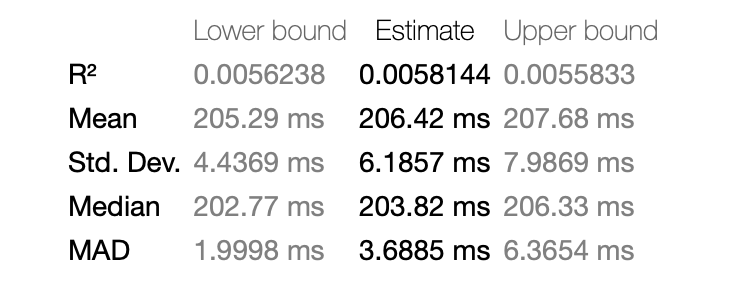
\includegraphics[width=0.40\textwidth]{images/benchmark/too_large_graph/benchmark_graph_500_24876_rust}
    \caption{Result benchmark Rust implementation}
    \label{fig:benchmark-graph-500-24876-rust}
\end{figure}

\subsubsection*{Benchmark Comparison}
\begin{figure}[!h]
    \centering
    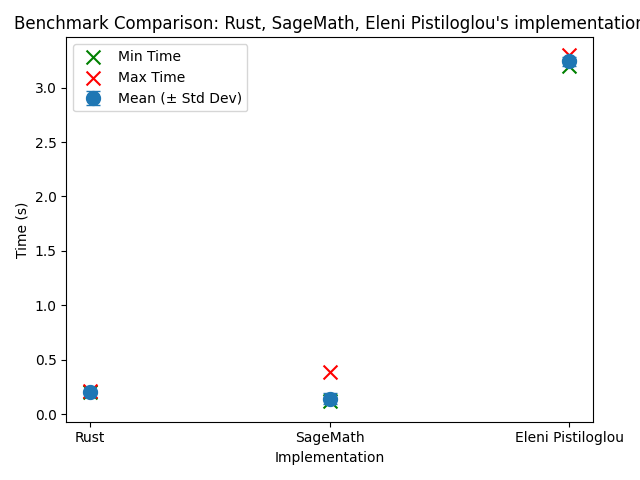
\includegraphics[width=0.40\textwidth]{images/benchmark/too_large_graph/benchmark_comparison_graph_500_24876}
    \caption{Result benchmark Rust implementation}
    \label{fig:benchmark-comparison-graph-500-24876}
\end{figure}


\newpage


\subsection{500 nodes - 24864 edges}\label{subsec:result-for-graphs-500-24864}

\subsubsection*{SageMath implementation}
\begin{figure}[!h]
    \centering
    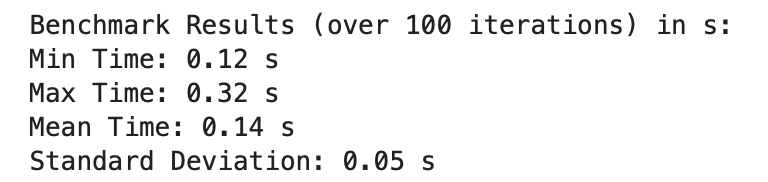
\includegraphics[width=0.60\textwidth]{images/benchmark/graph_500_24864/benchmark_graph_500_24864_sagemath}
    \caption{Result benchmark SageMath implementation}
    \label{fig:benchmark-graph-500-24864-sagemath}
\end{figure}

\subsubsection*{Eleni Pistiloglou's implementation}
\begin{figure}[!h]
    \centering
    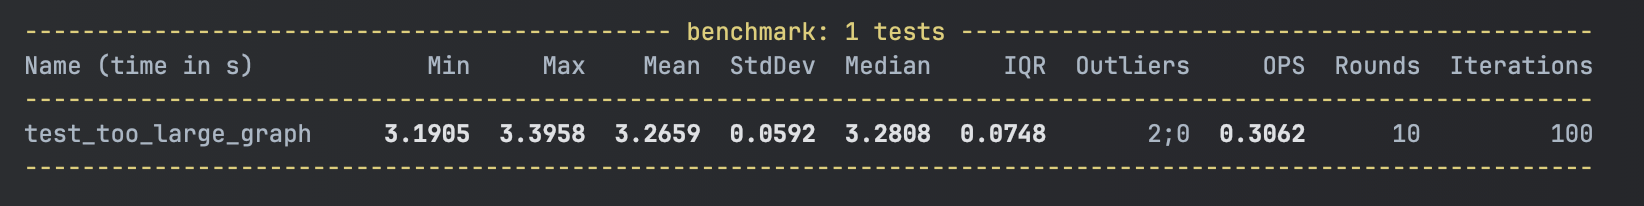
\includegraphics[width=0.60\textwidth]{images/benchmark/graph_500_24864/benchmark_graph_500_24864_python}
    \caption{Result benchmark Eleni Pistiloglou's implementation}
    \label{fig:benchmark-graph-500-24864-python}
\end{figure}

\subsubsection*{Rust implementation}
\begin{figure}[!h]
    \centering
    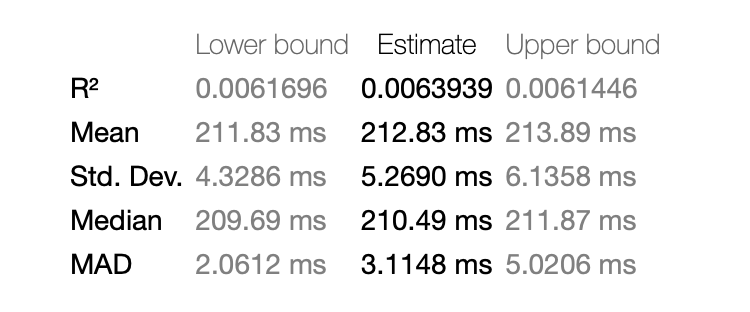
\includegraphics[width=0.40\textwidth]{images/benchmark/graph_500_24864/benchmark_graph_500_24864_rust}
    \caption{Result benchmark Rust implementation}
    \label{fig:benchmark-graph-500-24864-rust}
\end{figure}

\subsubsection*{Benchmark Comparison}
\begin{figure}[!h]
    \centering
    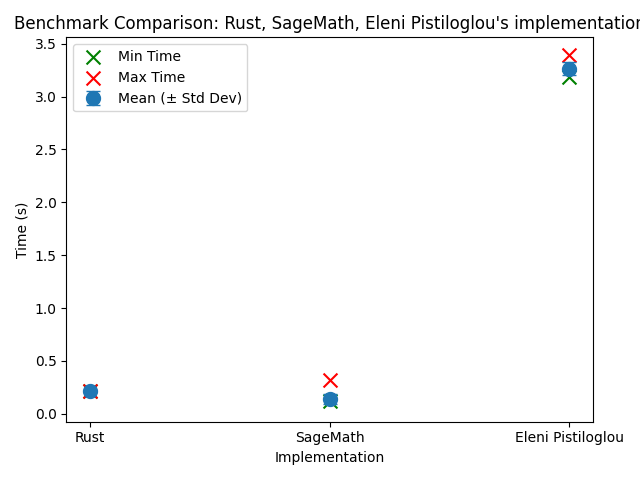
\includegraphics[width=0.40\textwidth]{images/benchmark/graph_500_24864/benchmark_comparison_graph_500_24864}
    \caption{Result benchmark Rust implementation}
    \label{fig:benchmark-comparison-graph-500-24864}
\end{figure}


\newpage


\subsection{800 nodes - 63378 edges}\label{subsec:result-for-graphs-800-63378}

\subsubsection*{SageMath implementation}
\begin{figure}[!h]
    \centering
    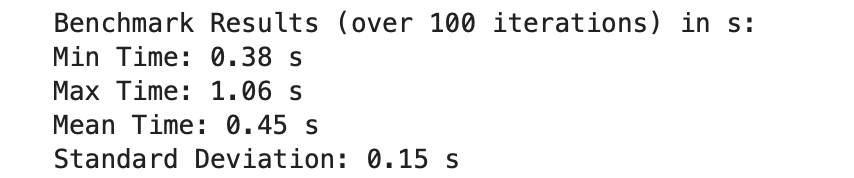
\includegraphics[width=0.40\textwidth]{images/benchmark/graph_800_63378/benchmark_graph_800_63378_sagemath}
    \caption{Result benchmark SageMath implementation}
    \label{fig:benchmark-graph-800-63378-sagemath}
\end{figure}

\subsubsection*{Eleni Pistiloglou's implementation}
\begin{figure}[!h]
    \centering
    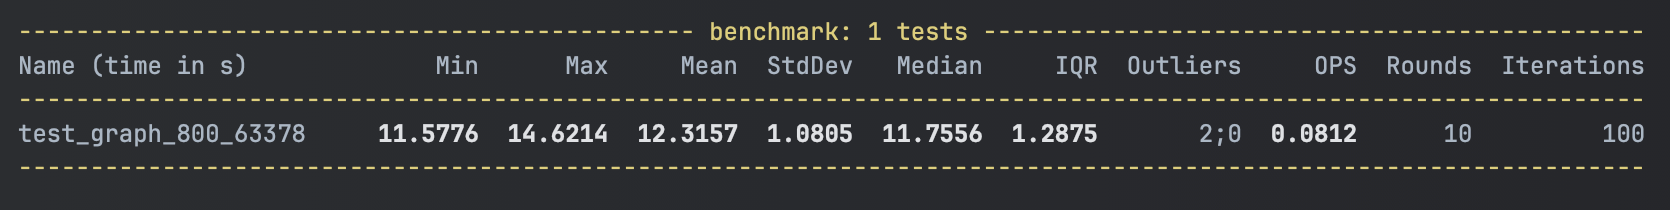
\includegraphics[width=0.60\textwidth]{images/benchmark/graph_800_63378/benchmark_graph_800_63378_python}
    \caption{Result benchmark Eleni Pistiloglou's implementation}
    \label{fig:benchmark-graph-800-63378-python}
\end{figure}

\subsubsection*{Rust implementation}
\begin{figure}[!h]
    \centering
    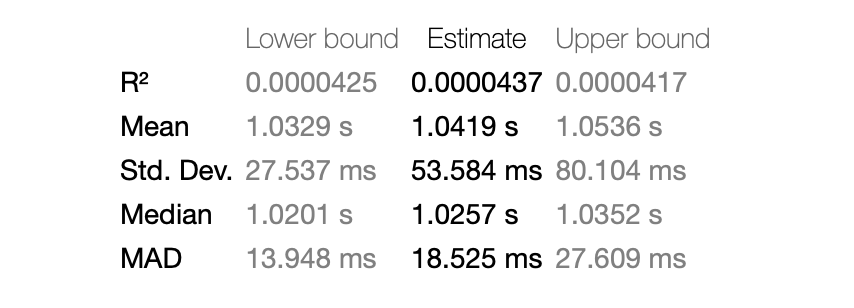
\includegraphics[width=0.40\textwidth]{images/benchmark/graph_800_63378/benchmark_graph_800_63378_rust}
    \caption{Result benchmark Rust implementation}
    \label{fig:benchmark-graph-800-63378-rust}
\end{figure}

\subsubsection*{Benchmark Comparison}
\begin{figure}[!h]
    \centering
    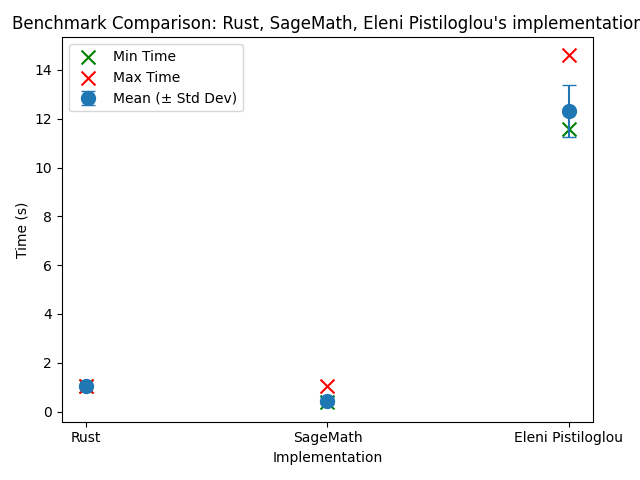
\includegraphics[width=0.40\textwidth]{images/benchmark/graph_800_63378/benchmark_comparison_graph_800_63378}
    \caption{Result benchmark Rust implementation}
    \label{fig:benchmark-comparison-graph-800-63378}
\end{figure}

\newpage


\subsection{1000 nodes - 100206 edges}\label{subsec:result-for-graphs-1000-100206}

\subsubsection*{SageMath implementation}
\begin{figure}[!h]
    \centering
    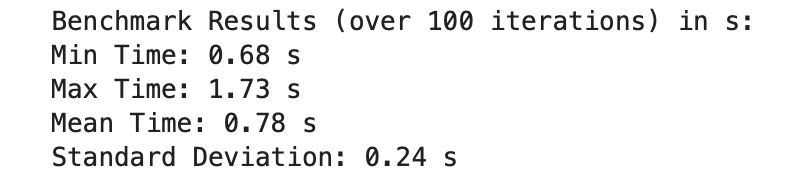
\includegraphics[width=0.80\textwidth]{images/benchmark/graph_1000_100206/benchmark_graph_1000_100206_sagemath}
    \caption{Result benchmark SageMath implementation}
    \label{fig:benchmark-graph-1000-100206-sagemath}
\end{figure}


\subsubsection*{Rust implementation}
\begin{figure}[!h]
    \centering
    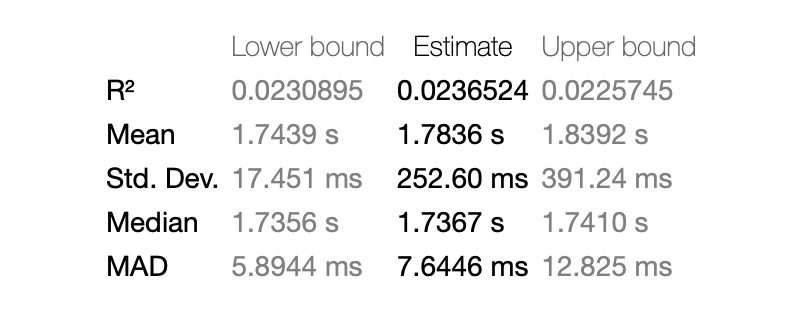
\includegraphics[width=0.80\textwidth]{images/benchmark/graph_1000_100206/benchmark_graph_1000_100206_rust}
    \caption{Result benchmark Rust implementation}
    \label{fig:benchmark-graph-1000-100206-rust}
\end{figure}

\subsubsection*{Benchmark Comparison}
\begin{figure}[!h]
    \centering
    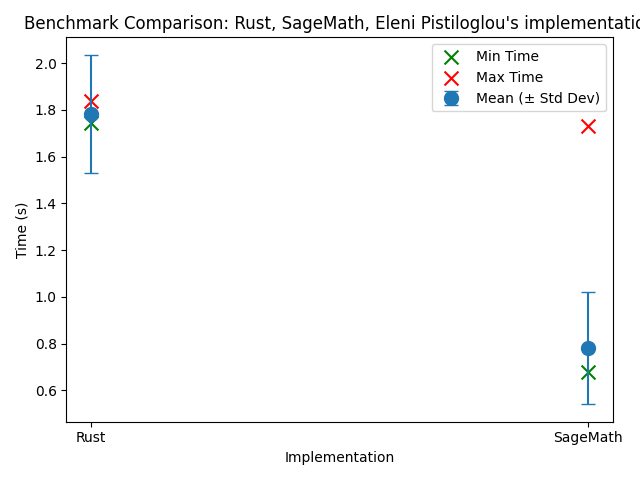
\includegraphics[width=0.40\textwidth]{images/benchmark/graph_1000_100206/benchmark_comparison_graph_1000_100206}
    \caption{Result benchmark Rust implementation}
    \label{fig:benchmark-comparison-graph-1000-100206}
\end{figure}


\newpage

\section{Conclusion}\label{sec:conclusion}

The benchmark results show that implementations of modular decomposition algorithms in SageMath, Eleni Pistiloglou's version in Python and Rust exhibit significant performance differences as a function of graph size and structure.

\begin{itemize}
    \item Small graphs: For small graphs, all implementations are efficient with minor differences in execution time.
    The Python and SageMath implementations gave comparable results, although SageMath was slightly faster.
    \item Large graphs: As the size of the graph increased, particularly for graphs containing hundreds of nodes and thousands of edges, the performance differences became pronounced.
    Rust always outperformed Python, thanks to its memory management and concurrency capabilities, but was falling behind SageMath.
    Python was the slowest performer, particularly when manipulating large graphs with complex structures, while SageMath performed moderately well, but often worse than Rust in some cases.
\end{itemize}

Overall, Rust offered good scalability and efficiency, particularly for smaller graphs.
SageMath, although slower, was better for larger and more complex graphs, and the Eleni Pistiloglou's implementation in Python, although flexible and easy to understand, struggled to perform on a large scale.
